% LREC 2026 Example; 
% LREC Is now using templates similar to the ACL ones. 
\documentclass[10pt, a4paper]{article}

\usepackage[review]{lrec2026} % this is the new style
\usepackage{natbib} 
\usepackage{amsmath} % for \text in math mode
\usepackage{amssymb} % for \mathbb
\usepackage{algorithm}
\usepackage{algpseudocode}
\let\oldtexttt\texttt
\renewcommand{\texttt}[1]{{\small\oldtexttt{#1}}}
% the 'review' option anonymizes the paper following submission guideline
% the 'final' option produces the camera ready version (non anonymized)
% default version is 'final', so use review option for submission

\title{Inference-Time Complexity Control for Small Language Models in Educational Applications}

\name{Santiago Robaina, Aiala Rosá, Luis Chiruzzo} 

\address{Affiliation1, Affiliation2, Affiliation3 \\
         Address1, Address2, Address3 \\
         author1@xxx.yy, author2@zzz.edu, author3@hhh.com\\
         \{author1, author5, author9\}@abc.org\\}


\abstract{
Small Language Models (SLMs) deployed in educational settings must generate text appropriate for beginner learners, yet they typically produce responses far exceeding A1-level proficiency. We investigate two lightweight, training-free inference-time interventions---contextual prompting and A1 vocabulary probability weighting---for controlling text complexity in SLMs (0.5B--3.8B parameters), targeting resource-constrained educational deployments where retraining is infeasible. A 2$\times$2 factorial experiment across four model architectures (Qwen2.5, Qwen3, Phi3, TinyLlama) and 15 A1-level prompts reveals that contextual prompting is the dominant mechanism, achieving 27--47\% complexity reductions across all readability metrics, while standalone vocabulary weighting shows minimal impact. Intervention effectiveness is highly architecture-dependent, with interaction effects ranging from negative (Qwen2.5) to strongly positive (Qwen3). Human evaluation of the top configurations exposes a practitioner trade-off: Qwen3 achieves highest simplicity but Phi3 scores higher on correctness and naturalness, highlighting the limits of automatic readability metrics for educational deployment decisions.
\newline \Keywords{Small Language Models, Text Complexity Control, Readability Metrics, Educational NLP, Inference-Time Control} }

\begin{document}

\maketitleabstract
\section{Introduction}
Language learning applications increasingly rely on AI assistants to provide personalized instruction and practice opportunities. However, a critical challenge emerges when deploying these systems for beginner learners: pretrained language models typically generate text that exceeds the linguistic proficiency of early-stage learners. Consider the following example from a small language model responding to an A1-level English learner:

Prompt:\texttt{ "What is a `friend'?"}

Control (Phi3-mini, no interventions):

\texttt{"A friend is a person with whom one shares a bond of mutual affection, trust, and support. Friendships are often formed due to shared experiences, interests, or values, and they can provide emotional comfort, companionship, and a sense of belonging. Friends typically enjoy spending time together, engaging in activities, and offering each other advice or assistance when needed. Friendships can be formed at any stage in life and play a crucial role in personal and social development."}

Interventions (Phi3-mini, prompting + weighting):

\texttt{"A friend is a person who you like and enjoy spending time with. Friends play with you, talk to you, and help you when you need it. You can have many friends, and they can be people who live close to you or people who you know from school or a club. Friends make you feel happy and safe."}

The uncontrolled response, while semantically accurate, uses vocabulary and sentence structures far beyond A1-level proficiency (Flesch-Kincaid Grade 12.0, 29 difficult words).
The combined intervention reduces this to Grade 2.8 with only 1 difficult word, while preserving the factual content of the answer.
The complexity mismatch limits the pedagogical value of AI-assisted language learning, as learners cannot understand the responses intended to help them.

Existing approaches to controlling text complexity face significant limitations for educational deployments: All require substantial resources and lack flexibility

% Fine-tuning methods require substantial computational resources, labeled training data, and lock models into fixed complexity levels determined during training. Recent decoding-time control methods demonstrate promising results but require training auxiliary models (expert models, predictors, or discriminators) and focus predominantly on large language models requiring cloud infrastructure. Critically, no prior work addresses inference-time complexity control for small language models through lightweight, training-free mechanisms suitable for resource-constrained educational contexts.

This work is conducted within a larger project developing conversational agents for educational purposes, focusing on beginner English learners with minimal prior experience. The emphasis on Small Language Models \cite{fang2024survey} in the 0.5-3.8B parameter range, rather than large proprietary models emerges from deployment constraints: on-device inference eliminates cloud costs and enables offline functionality, critical for resource-constrained educational institutions with variable connectivity.

We present a method that combines contextual prompting with probability weighting via vocabulary-aware logits processors, enabling inference-time complexity control without model retraining or auxiliary model training. The methodology applies soft constraints through probability boosting for target vocabulary tokens from the Cambridge A1 "Starters" curriculum (494 words), guiding models toward simpler alternatives while preserving generation flexibility.

In the following section, the paper covers the related work reviewing existing approaches to complexity control. Then the methods section presents the experimental design. The results section reports aggregate performance across models and compares model specific results in prompting versus combined interventions. The discussion interprets our findings, synthesizing key contributions . The paper concludes and acknowledges limitations and presents an ethics statement.


\section{Related Work}

\subsection{Linguistic Complexity Control}

Training-time approaches for controlling linguistic complexity span data curation, fine-tuning,
and architecture-level control.
\citet{eldan2023tinystories} showed that restricting training vocabulary to words understood
by 3--4 year-olds produces narratives with controlled lexical complexity, but fixes complexity
at training time.
\citet{nguyen2024multi} introduced MCTune, which embeds target complexity values into LLaMA2-7B
instruction tuning, achieving multi-dimensional control while maintaining coherence.
\citet{nie2023lexical} embed complexity representations directly into the model architecture and
enforce sentence-length and syntactic constraints during decoding.
\citet{tran2024readctrl} instruction-tune Mistral-7B on readability-augmented data, enabling
generation at near-continuous complexity targets.
\citet{malik2024tarzan} demonstrate that prompt-only strategies leave a large gap between GPT-4
and smaller open-source models, and that fine-tuning with reinforcement learning alignment
closes it.
All five methods require substantial computational resources, labeled training data, and fix
complexity targets at training time, offering no mechanism for dynamic adaptation to individual
learner proficiency.\textbf{}

\subsection{Decoding-Time Control through Probability Manipulation}

\citet{liu2021dexperts} introduced DExperts, which steers generation by adjusting token logits
according to the difference between expert and anti-expert model predictions.
\citet{yang2021fudge} train a future discriminator that predicts attribute satisfaction from
partial sequences and multiplies its output into the base model's token probabilities at each
step.
Both methods enable inference-time control without retraining the base model, but require
training auxiliary models and target general attributes (toxicity, sentiment, formality) rather
than linguistic complexity for educational applications.

\subsection{Research Gap and Contributions}

Training-time methods provide precise control but require retraining and lock complexity targets
at training time; decoding-time methods (DExperts, FUDGE) avoid retraining but require learned
auxiliary models and do not address linguistic complexity for resource-constrained, sub-4B
deployments.
This work combines inference-time contextual prompting with direct A1 vocabulary probability
amplification via a predefined word list, requiring neither model retraining nor auxiliary model
training.

\section{Method}
The experimental setup is presented next, describing the evaluated models and configurations as well as the proposed interventions.

\subsection{Experimental design}
A factorial experiment was conducted to systematically evaluate the effectiveness of two inference-time interventions for controlling text complexity in Small Language Models. The experimental design was the following:
\begin{itemize}
    \item \textbf{Models (4):}
    \begin{itemize}
        \item Phi-3-mini (3.8B) \cite{abdin2024phi3}
        \item Qwen2.5 (0.5B) \cite{qwen2024qwen25}
        \item Qwen3 (0.6B) \cite{qwen2025qwen3}
        \item TinyLlama (1.1B) \cite{zhang2024tinyllama}
    \end{itemize}
    \item \textbf{System prompt:} 
    
    \texttt{``You are a helpful English teacher for beginner students.} 
    
    \texttt{Answer with a paragraph only with plain text.''}
    \item \textbf{Intervention Conditions (4):} 
    \begin{enumerate}
        \item Control: No interventions applied
        \item Weighting Only: Probability boosting via vocabulary list
        \item Prompting Only: Contextual instructions for simplification
        \item Both: Combined weighting and prompting
    \end{enumerate}
    \item Test Prompts (15): Diverse English learning scenarios covering vocabulary definitions, self-introduction, basic concepts, comparisons, descriptions, and daily activities
\end{itemize}

This $4 \times 4 \times 15$ factorial design spans 240 total observations, enabling systematic analysis of main effects (weighting, prompting), interaction effects (weighting × prompting), and model-specific differences.

\subsubsection{Model selection}
The selected models span a parameter range from 0.5B to 3.8B, representing the current landscape of deployable Small Language Models suitable for on-device inference. All models were evaluated using quantized 4-bit GGUF format implementations, ensuring consistent evaluation conditions and realistic deployment performance characteristics. Model selection prioritized parameter efficiency (<4B parameters), architectural diversity (Qwen, Llama, Phi families) and instruction-following capability.

\subsubsection{Prompt design}
The 15 test prompts represent A1-level English conversation scenarios across four categories: Vocabulary Definitions (5 prompts, e.g., ``What does the word `library' mean?''), Conceptual Explanations (4 prompts, e.g., ``What is a dog?''), Comparative Questions (2 prompts, e.g., ``What is the difference between `big' and `large'?''), and Descriptive Tasks (4 prompts, e.g., ``What colors do you see in a rainbow?''). All prompts were designed to elicit paragraph-length responses (30--100 words) suitable for evaluating readability metrics.

\subsection{Intervention Methodologies}
\subsubsection{Probability Weighting Intervention}
The probability weighting intervention implements soft vocabulary constraints through inference-time manipulation of token generation probabilities during the decoding process. The mechanism operates as follows:

\textbf{Vocabulary Selection}: A target vocabulary was compiled from the Cambridge English A1 "Starters word list", comprising 494 word entries including basic words (e.g., "happy", "dog", "school"). This vocabulary represents the expected lexical knowledge of A1-level English learners. Special tokens, like end tokens (\texttt{<|im\_end|>,<|endoftext|>}), were included in the list to avoid long answers due to this weighting.

\textbf{Token-Level Weighting}: Each word in the vocabulary is tokenized using the model's tokenizer, producing one or more subword tokens depending on the model's vocabulary. The weighting intervention operates at the token level: bias values are applied to the token IDs resulting from this tokenization process, not to whole words directly. For example, the word "afternoon" may tokenize to ["after", "noon"], and both resulting token IDs receive the weight bias. Crucially, the boost is applied at \emph{every} decoding step: when a multi-token word spans several steps, each constituent sub-token independently receives the additive bias. Algorithm~\ref{alg:weighting} summarises the per-step procedure. Adding $\log(\alpha)$ in log-space is equivalent to multiplying the token's probability by $\alpha$ before renormalisation, which is the standard soft-constraint logits-processor pattern.

\begin{algorithm}[h]
\caption{Vocabulary Probability Weighting (per decoding step)}
\label{alg:weighting}
\begin{algorithmic}[1]
\Require $\text{logits} \in \mathbb{R}^{|V|}$ \ (raw token scores at each decoding step)
\Require $V_{A1}$ \ (set of token IDs from A1 vocabulary); $\alpha = 1.5$ \ (boost factor)
\For{each decoding step}
    \For{$\text{token\_id} \in V_{A1}$}
        \State $\text{logits}[\text{token\_id}] \mathrel{+}= \log(\alpha)$ \hfill $\triangleright$ multiply probability by $\alpha$ before renorm.
    \EndFor
    \State $\text{next\_token} \gets \text{sample}\!\left(\text{softmax}(\text{logits})\right)$
\EndFor
\end{algorithmic}
\end{algorithm}


\subsubsection{Basic weight exploration}
A supplementary experiment evaluated three multiplicative factors ($1.5\times$, $2.0\times$, $4.0\times$) in the weighting-only condition across all four models and 15 prompts (172 valid responses). $1.5\times$ achieved the lowest mean FK Grade (8.76) and highest output stability (SD\,=\,3.23), while $4.0\times$ paradoxically increased complexity (FK 13.85, SD\,=\,13.04), suggesting excessive constraints trigger compensatory verbosity; $1.5\times$ was therefore selected for all experiments.

\subsubsection{Context prompting intervention}
The prompting intervention provides explicit instructions to guide the model toward generating simpler, more accessible text. The intervention consists in appending a context instruction to each user query:
``\texttt{\# Context}

\texttt{Please respond using simple words that a young non-English speaking student can understand.} 

\texttt{Use vocabulary from basic English learning materials. Keep sentences short and clear.}

\texttt{Avoid complex grammar structures and difficult words.}
''


The context prompt establishes explicit simplification constraints: audience specification ("young non-English speaking student") sets the tone for complexity adjustment, vocabulary constraint ("simple words", "basic English learning materials") guides lexical selection, sentence structure directive ("short and clear") targets syntactic simplification, and grammar constraint ("avoid complex structures") prevents advanced formulations.


\subsection{Metrics}
Two types of metrics were selected for complexity evaluation: primary readability metrics and
secondary count metrics that provide reference information on generation characteristics.
All primary metrics are ascending in complexity; lower values are the target in this work.

\subsubsection{Primary Readability Metrics}

\textbf{Flesch-Kincaid Grade Level} \cite{kincaid1975derivation} estimates U.S. school grade
level from average sentence length and average syllables per word.
It is the most widely adopted readability measure in educational contexts.
Target for A1 learners: $\leq 5.0$ (elementary level).

\textbf{Gunning Fog Index} \cite{gunning1952technique} combines sentence length with the
proportion of polysyllabic words ($\geq$3 syllables), making it particularly sensitive to
complex vocabulary.
Target: $\leq 6.0$ (sixth grade or below).

\textbf{SMOG Index} \cite{mclaughlin1969smog} estimates reading level from the raw count of
polysyllabic words, with lower sensitivity to sentence length than Flesch-Kincaid.
It is specifically designed for short texts.
Target: $\leq 7.0$ (junior high or below).

\textbf{Spache Readability} \cite{spache1953new} combines sentence length with the proportion
of words outside a reference list of ~1,000 common primary-grade words, providing finer
discrimination at low proficiency levels.
Target: $\leq 4.0$ (primary grades).

\subsubsection{Secondary Descriptive Metrics}

\textbf{Word Count} and \textbf{Difficult Words Count} (words absent from the Dale-Chall easy
word list \cite{dale1948formula}) provide directly interpretable measures of response length
and vocabulary accessibility.


% \textbf{A1 target ranges:} Table~\ref{tab:a1-targets} shows the target ranges for successful A1-level text generation across primary metrics and secondary statistics.

% \begin{table}
% \centering
% \small
% \begin{tabular}{lll}
% \hline
% \textbf{Metric} & \textbf{Target} & \textbf{Interpretation}\\
% \hline
% \multicolumn{3}{l}{\textit{Primary Metrics}} \\
% Flesch-Kincaid Grade & $\leq 5$ & $\leq$ Elementary \\
% Gunning Fog & $\leq 6$ & $\leq$ Sixth grade \\
% SMOG Index & $\leq 7$ & $\leq$ Junior high \\
% Spache Readability & $\leq 4$ & Primary grades \\
% \hline
% \end{tabular}
% \caption{\label{tab:a1-targets} Target ranges for A1 English learner text generation. Primary metrics assess readability complexity; secondary statistics measure response characteristics.}
% \end{table}

\subsubsection{Human Evaluation}
To complement automatic readability metrics, a human evaluation was conducted on the subset of configurations that achieved the best automatic complexity scores. The evaluation covered the top four configurations by a composite normalized metric: \textit{Phi3-prompted}, \textit{Phi3-weighted+prompted}, \textit{Qwen3-prompted}, and \textit{Qwen3-weighted+prompted} (60 responses total, 15 per configuration). Three annotators rated each response on a 1--5 scale across three dimensions:
\begin{itemize}
    \item \textbf{Correctness}: factual accuracy and completeness of the response
    \item \textbf{Simplicity}: appropriateness of vocabulary and sentence structure for young A1 learners
    \item \textbf{Naturalness}: fluency and coherence of the generated text
\end{itemize}
The identity of the model was anonymized and the rows were randomized to prevent bias from the evaluation.

\subsubsection{Computational environment} All experiments ran on a MacBook Pro M2 (2022, 8-core CPU, 8GB unified memory) using llama-cpp-python ($\geq$0.2.0) with Python 3.12 for GGUF inference and textstat ($\geq$0.7.3) for readability computation. All models used identical decoding settings: temperature 0.7, top-$k$ 50, top-$p$ 0.95, maximum 200 output tokens, no repetition penalty. Phi3 used Metal Performance Shaders (MPS) for full GPU offload; the remaining models ran on CPU.

\section{Results}
The results show a clear heterogeneity over the different models, an aggregate performance analysis is used to observe the clear impact of prompt-based interventions. To study the effects of weighting added to the prompting intervention, a model specific case study shows this clear variety of results depending on the model

\subsection{Aggregate Performance Across Models}

Tables~\ref{tab:table1a} and~\ref{tab:table1b} present the median performance metrics aggregated across all four models (n=60 per configuration). The control condition established baseline complexity levels considerably higher than A1 target thresholds across all metrics (Flesch-Kincaid Grade Level [FK], Gunning Fog Index [GF], SMOG, Spache[Spa.]). Prompting-based interventions ("Prompting Only" and "Both") achieved substantial reductions of 27-47\% across all readability measures. In contrast, standalone vocabulary weighting showed minimal impact on complexity, accompanied by a 7\% increase in word count.

\begin{table}[!ht]
\begin{center}
\begin{tabular}{lcccc}
\hline
\textbf{Config.} & \textbf{FK} & \textbf{GF} & \textbf{SMOG} & \textbf{Spa.} \\
\hline
Control   & 9.13  & 10.98 & 11.55 & 5.08 \\
Weighting & 9.47  & 11.33 & 11.21 & 5.31 \\
Prompting & 4.84* & 6.09  & 8.16  & 3.29* \\
Both      & 4.93* & 6.72  & 8.68  & 3.54* \\
\hline
\end{tabular}
\caption{Primary Readability Metrics by Configuration (All Models Combined, n=60). *Meets A1 target (FK $\leq$ 5.0; Spache $\leq$ 4.0)}
\label{tab:table1a}
\end{center}
\end{table}

\begin{table}[!ht]
\begin{center}
\begin{tabular}{lcc}
\hline
\textbf{Config.} & \textbf{Words} & \textbf{Diff. Words} \\
\hline
Control   & 83.5 & 15.0 \\
Weighting & 89.5 & 14.5 \\
Prompting & 63.5 & 4.0  \\
Both      & 60.5 & 4.0  \\
\hline
\end{tabular}
\caption{Secondary Metrics by Configuration (All Models Combined, n=60)}
\label{tab:table1b}
\end{center}
\end{table}

The combined intervention ("Both") demonstrated negligible benefit over prompting alone across all primary metrics. This suggests that contextual prompting captures the majority of achievable simplification. When adding weighting, the result was 5\% fewer words with no change in difficult word count, indicating that the intervention primarily affects response length rather than vocabulary selection. Difficult words were reduced by 73\% under prompting interventions, directly addressing vocabulary accessibility requirements for A1 learners.

\begin{figure}[!ht]
\begin{center}
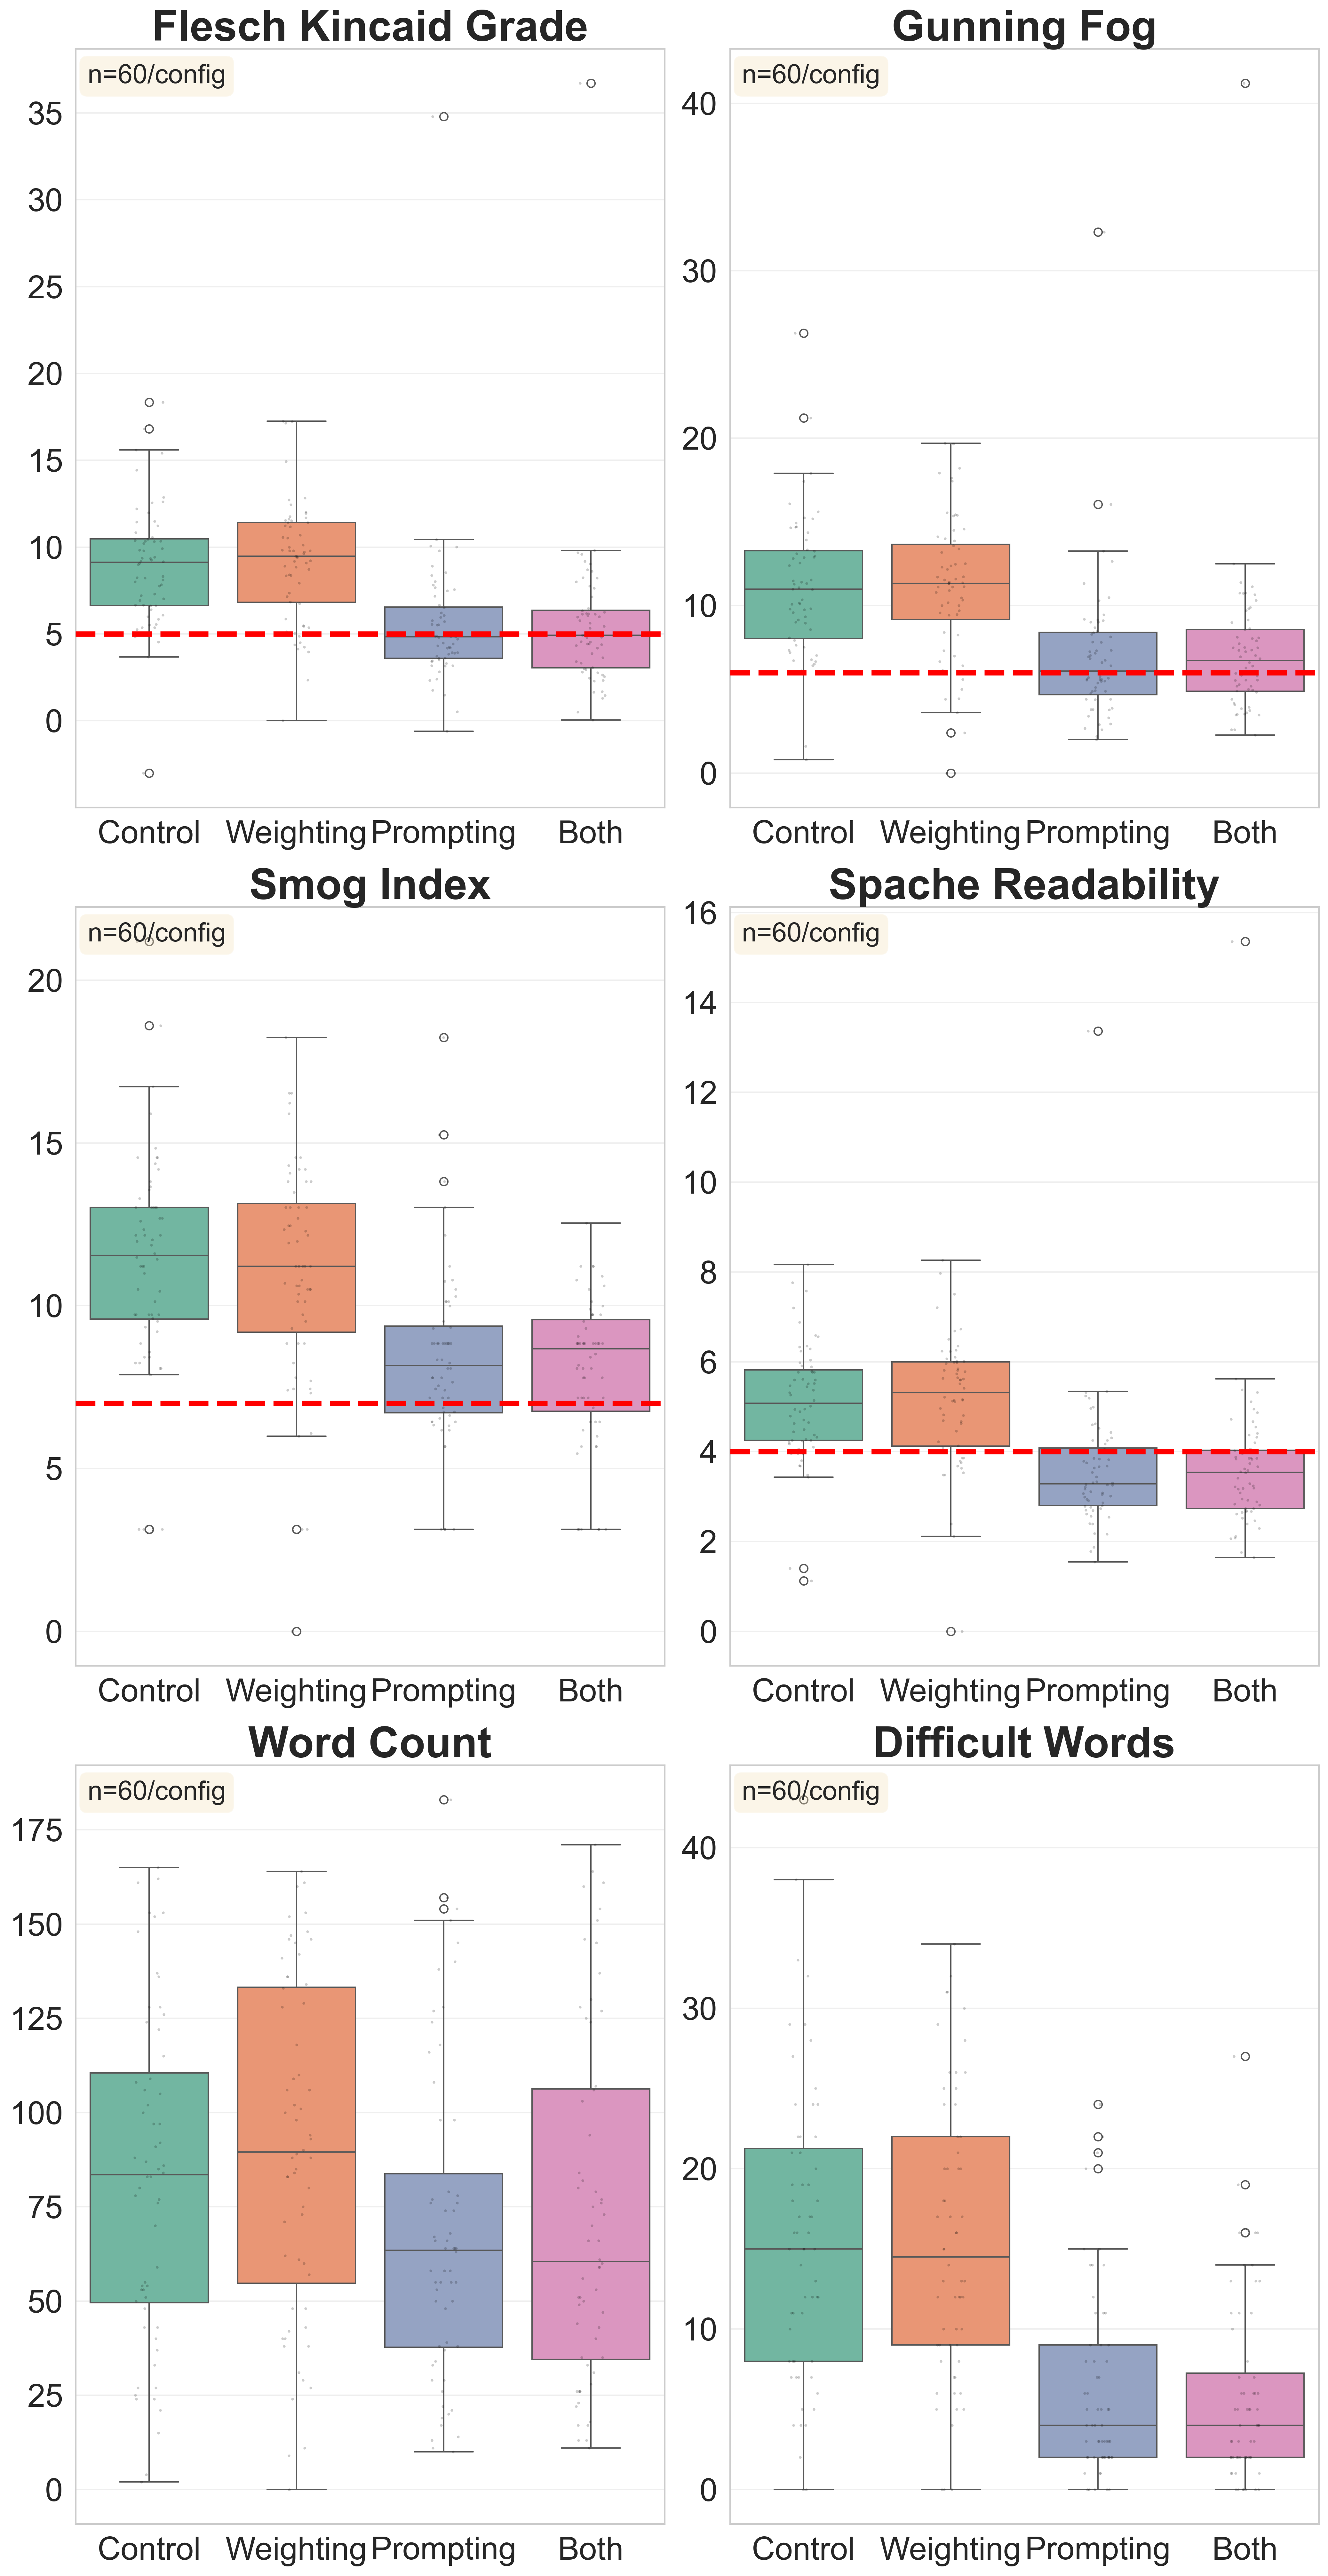
\includegraphics[width=\columnwidth]{plots/aggregate_all_models_1023_2345.png}
\caption{Aggregate Performance Distributions Across All Models. The red line indicates the target value}
\label{fig:aggregate}
\end{center}
\end{figure}

Figure~\ref{fig:aggregate} presents boxplot distributions of all readability metrics aggregated across the four models (n=60 per configuration). The visualizations confirm the substantial separation between control/weighting conditions and prompting-based interventions across all metrics. Prompting configurations demonstrate consistently lower complexity with reduced variance, while standalone vocabulary weighting shows minimal aggregate change from control with higher variability. The combined intervention exhibits similar central tendencies to prompting alone, with minimal additional benefit visible across all six metrics.

\subsection{Prompting vs Combined Intervention Analysis}

Table~\ref{tab:table2} quantifies the marginal contribution of vocabulary weighting when combined with prompting, given the minimal aggregate impact of standalone weighting (Section~4.1).

\begin{table}[!ht]
\begin{center}
\begin{tabular}{llccc}
\hline
\textbf{Model} & \textbf{Metric} & \textbf{Both} & \textbf{$\Delta$} & \textbf{$\Delta$\%} \\
\hline
Phi3      & FK          & 3.41 & -0.83 & -19.6  \\
          & GF          & 5.55 & +0.08 & +1.5  \\
          & SMOG        & 7.17 & -0.48 & -6.3  \\
          & Spa.        & 2.83 & -0.11 & -3.7  \\
          & Words       & 66.0 & 0.0  & 0.0  \\
          & Difficult & 3.0  & 0.0  & 0.0  \\
\hline
Qwen2.5   & FK          & 6.34  & +0.62 & +10.8 \\
          & GF          & 8.11 & +0.78 & +10.6 \\
          & SMOG        & 8.84  & 0.0 & 0.0  \\
          & Spa.        & 4.02  & +0.20 & +5.2 \\
          & Words       & 61.0  & +3.0  & +5.2 \\
          & Difficult & 5.0   & 0.0  & 0.0 \\
\hline
Qwen3     & FK          & 2.80 & -0.92 & -24.7  \\
          & GF          & 3.85 & -0.92 & -19.3  \\
          & SMOG        & 7.17 & -0.28 & -3.8  \\
          & Spa.        & 2.81 & -0.05 & -1.7  \\
          & Words       & 26.0 & -12.0  & -31.6 \\
          & Difficult & 2.0  & 0.0  & 0.0  \\
\hline
TinyLlama & FK          & 5.98  & -1.20 & -16.7 \\
          & GF          & 9.0  & +0.55 & +6.5 \\
          & SMOG        & 9.73  & +0.21 & +2.2  \\
          & Spa.        & 4.01  & +0.01 & +0.3 \\
          & Words       & 124.0  & +50.0 & +67.6 \\
          & Difficult & 11.0   & 0.0   & 0.0   \\
\hline
\end{tabular}
\caption{Marginal Effect of Adding Weighting to Prompting ($\Delta$ = Both - Prompting Only)}
\label{tab:table2}
\end{center}
\end{table}

\subsubsection{Model-Specific Interaction Patterns}


\textbf{Phi3 (3.8B)} demonstrated positive complementary effects between interventions, with the combined intervention achieving a $20\%$ FK reduction beyond prompting alone. The intervention maintained identical word count and difficult word count to prompting alone, indicating efficient complexity reduction without compensatory verbosity or vocabulary substitution effects.

\textbf{Qwen2.5 (0.5B)} exhibited a negative interaction, with the combined intervention underperforming prompting alone across primary readability metrics. This represents an $11\%$ increase in FK complexity when adding vocabulary weighting to prompting. The intervention triggered modest compensatory verbosity ($5\%$ word count increase) with no change in difficult word count. This pattern suggests fundamental architectural incompatibility between vocabulary constraints and instruction-following in this model.

\textbf{Qwen3 (0.6B)} demonstrated strong positive interaction across most metrics, achieving the lowest absolute complexity of any configuration tested (FK: 2.80). The combined intervention achieved a $25\%$ FK reduction beyond prompting alone while dramatically reducing word count by $32\%$, indicating efficient simplification without compensatory verbosity. This model's unique responsiveness to standalone vocabulary weighting (the only model achieving A1 targets with weighting alone) suggests that its training data or architectural design predisposes it to benefit from lexical constraints.

\textbf{TinyLlama (1.1B)} exhibited positive interaction for FK complexity, representing a $17\%$ reduction when adding vocabulary weighting to prompting. However, TinyLlama exhibited severe compensatory verbosity with a $68\%$ word count increase and no reduction in difficult word count, indicating that the complexity reduction follows from syntactic restructuring rather than vocabulary substitution. Despite this positive interaction, no configuration achieved A1 targets.

\subsubsection{Aggregate Trade-off Analysis}

Across all models, the combined intervention produced $5\%$ fewer words than prompting alone with no change in difficult word count. However, this aggregate pattern masks substantial model-level heterogeneity. The effectiveness of vocabulary weighting when combined with prompting is highly model-dependent:

 \begin{itemize}
     \item \textbf{Beneficial} (Qwen3, Phi3, TinyLlama): Vocabulary constraints yield net complexity reduction, with Qwen3 achieving word count reduction ($32\%$), Phi3 showing efficient complexity reduction without verbosity changes, and TinyLlama reducing FK complexity despite severe verbosity ($68\%$ increase)
     \item \textbf{Detrimental} (Qwen2.5): Compensatory verbosity triggers output instability and complexity increases across primary metrics
 \end{itemize}

These findings indicate that intervention effectiveness is highly model-dependent, with Qwen3 representing the configuration where vocabulary weighting provides the strongest benefits across all readability measures while dramatically reducing verbosity.

\subsection{Human Evaluation Results}

Table~\ref{tab:human-eval} presents average human ratings across the four best-performing configurations. Phi3 consistently outperformed Qwen3 on Correctness and Naturalness, while Qwen3 achieved higher Simplicity scores, aligning with its lower automatic readability values.

\begin{table}[!ht]
\begin{center}
\begin{tabular}{lccc}
\hline
\textbf{Config.} & \textbf{Correct.} & \textbf{Simple.} & \textbf{Natural.} \\
\hline
Phi3-P           & 4.18 & 3.18 & 4.16 \\
Phi3-W+P  & \textbf{4.40} & 3.38 & \textbf{4.45} \\
Qwen3-P          & 3.36 & 3.55 & 3.60 \\
Qwen3-W+P & 3.40 & \textbf{3.78} & 3.47 \\
\hline
\end{tabular}
\caption{Human Evaluation Results (1--5 scale, n=15 per configuration). Bold indicates best score per dimension. W: Weighted P: Prompted}
\label{tab:human-eval}
\end{center}
\end{table}

The results reveal a trade-off not captured by automatic metrics: Qwen3's higher simplicity comes at the cost of correctness and naturalness. Qualitative inspection identified two failure modes unique to Qwen3: (1) visible \texttt{<think>} reasoning tokens in several responses, indicating incomplete output filtering; and (2) semantically circular responses (e.g., defining ``big'' as ``large in size, but not necessarily so big''), which score well on readability formulas but poorly on human correctness judgement. Phi3's \textit{weighted+prompted} configuration achieved the best overall human evaluation profile, combining acceptable simplicity (3.38) with the highest correctness (4.40) and naturalness (4.45).

\subsubsection{Automatic Metric Alignment with Human Simplicity}

To assess whether automatic readability metrics reliably capture human simplicity perception, the configuration-level rankings were compared across metrics. The human simplicity ranking (Qwen3-W+P $>$ Qwen3-P $>$ Phi3-W+P $>$ Phi3-P) was compared against the orderings produced by each automatic metric. Flesch-Kincaid Grade achieved perfect rank agreement with human simplicity judgements across all four configurations. Gunning Fog closely matched human rankings, with only the two Phi3 configurations swapping positions (values of 5.69 vs.\ 5.60, a difference within natural variation). Spache Readability disagreed on the two Qwen3 configurations, ranking Qwen3-P as simpler than Qwen3-W+P, likely because Qwen3-W+P produces shorter but lexically denser responses that Spache penalizes more heavily. These results suggest that Flesch-Kincaid Grade and Gunning Fog Index are the most reliable proxies for perceived simplicity at the configuration level among the four readability metrics evaluated.

At the response level ($n=60$), Spearman correlations between automatic readability metrics and human simplicity ratings are moderate at best (Table~\ref{tab:metric-correlation}). Gunning Fog and Spache Readability show the strongest individual-response alignment ($\rho = -0.53$ and $\rho = -0.51$, respectively), while Flesch-Kincaid Grade achieves only weak-to-moderate response-level alignment ($\rho = -0.40$) and SMOG near-zero correlation ($\rho = -0.15$). All correlations are negative because readability formulas increase with complexity while human simplicity ratings increase with simplicity. Gunning Fog is the most consistent metric across both levels of analysis, while Flesch-Kincaid Grade's perfect configuration-level rank agreement does not extend to individual response assessment ($\rho = -0.40$), suggesting it is better suited for comparative system evaluation than per-response quality estimation. SMOG shows weak agreement at both levels and should not be treated as a reliable proxy for perceived simplicity. No automatic metric achieves strong alignment with human simplicity ratings at the individual response level, underscoring that human evaluation remains necessary for deployment decisions.

\begin{table}[!ht]
\begin{center}
\begin{tabular}{lc}
\hline
\textbf{Metric} & \textbf{Spearman $\rho$} \\
\hline
FK   & $-0.40$ \\
GF   & $-0.53$ \\
SMOG & $-0.15$ \\
Spa. & $-0.51$ \\
\hline
\end{tabular}
\caption{Spearman correlation between automatic readability metrics and human simplicity ratings at the response level ($n=60$). Negative values reflect that higher complexity scores correspond to lower human simplicity ratings.}
\label{tab:metric-correlation}
\end{center}
\end{table}

\section{Discussion}
Two main points are visible regarding the impact of the control mechanisms used: the effects on primary metrics, and the unwanted effect of verbosity generated on the weighting scenario. A third point concerns the reliability of automatic readability metrics as proxies for human-judged simplicity.

\subsection{Implications of Intervention Mechanisms}

The experimental results reveal two main insights for inference-time complexity control in Small Language Models.

\subsubsection{Instruction-Following as Primary Control Mechanism}

The dominance of contextual prompting over vocabulary weighting suggests that instruction-tuned models exhibit stronger responsiveness to high-level semantic constraints than low-level probability manipulation.

The minimal aggregate benefit of combining interventions (5\% fewer words, no change in difficult words) indicates that prompting already captures most achievable simplification. This suggests that instruction-tuning creates strong semantic priors that are difficult to modulate through token-level probability adjustments alone. For practitioners, this implies that prompt engineering should be prioritized over decoding manipulation for complexity control tasks.

Human evaluation (§4.3) further shows that the choice of model architecture determines whether simplification comes at the expense of pedagogical quality.

\subsubsection{Architectural implications on Intervention Effectiveness}

The substantial heterogeneity in interaction patterns—ranging from negative (Qwen2.5: $+11\%$ FK) to positive (Qwen3: $-25\%$ FK)—challenges the assumption of universal controllability mechanisms. Three architectural factors appear to determine intervention responsiveness:

\textbf{1. Instruction-following capability.} Models with strong instruction-following (Phi3) show positive benefit from vocabulary weighting ($20\%$ FK reduction), while models with weak instruction-following (TinyLlama) exhibit positive interaction effects for FK but severe compensatory verbosity. This suggests that vocabulary constraints can enhance instruction-tuning when architecturally compatible, though may trigger compensatory mechanisms in weaker models.

\textbf{2. Training data composition.} Qwen3's unique positive response to standalone vocabulary weighting ($9\%$ FK reduction) and low absolute readability scores distinguish it from other tested architectures. However, human evaluation reveals that Qwen3's strong automatic metric performance partially reflects two failure modes: visible \texttt{<think>} reasoning tokens appearing in several responses (indicating incomplete output filtering from its chain-of-thought pre-training), and semantically circular definitions (e.g., defining ``big'' as ``large in size, but not necessarily so big'') that score well on readability formulas but are pedagogically ineffective. This suggests that certain pre-training regimes may predispose models to benefit from lexical constraints while simultaneously introducing quality failure modes that automatic readability metrics cannot detect.

\textbf{3. Architectural stability under constraints.} Qwen2.5's output instability and complexity increases under combined interventions suggest architectural limitations in handling conflicting generation constraints. This implies that not all small model architectures are suitable for multi-constraint generation tasks.

\subsection{Compensatory Verbosity as a Design Constraint}

The $7\%$ aggregate word count increase under standalone vocabulary weighting reveals a fundamental tension in constrained generation: when lexical choices are restricted without semantic guidance, models compensate through syntactic elaboration. This compensation represents a critical challenge for soft constraint satisfaction in language models.

The observation that Qwen3 resisted compensatory verbosity while TinyLlama exhibited severe ($68\%$) word count increases suggests that this behavior is not universal but architecture-dependent. This has important implications for vocabulary-based intervention design: lexical constraints must be paired with explicit contextual guidance to prevent compensatory sentence lengthening. Across the architectures tested, standalone vocabulary manipulation was insufficient to achieve A1-level complexity without explicit prompting, though the degree of insufficiency varied: Qwen3 showed meaningful FK reduction ($9\%$) with weighting alone, while the remaining models showed negligible or negative effects.

Notably, Qwen3's resistance to compensatory verbosity does not guarantee pedagogical quality, as evidenced by its lower human correctness and naturalness scores relative to Phi3 despite achieving the shortest, lowest-complexity outputs.

\subsection{Automatic Metric Reliability for Educational Deployment}
The correlation analysis (Table~\ref{tab:metric-correlation}) shows that no automatic metric achieves strong individual-response alignment with human simplicity, with Gunning Fog being the most consistent proxy across both configuration-level and response-level analysis, and SMOG the least reliable ($\rho=-0.15$). A deeper limitation is illustrated by Qwen3's failure modes: circular definitions receive low readability scores while human annotators penalize them for correctness and naturalness, revealing that readability formulas cannot detect semantic quality failures. Human evaluation therefore remains necessary when selecting configurations for educational deployment.


\section{Conclusion}

This study demonstrates the viability of inference-time complexity control for Small Language Models in educational applications, with two key contributions:

\textbf{1. Understanding of intervention mechanisms:} Contextual prompting operates through high-level semantic constraints that leverage instruction-tuning, while vocabulary weighting provides low-level probability manipulation that shows architecture-dependent effects. The minimal aggregate benefit of combining interventions (5\% fewer words, no change in difficult words) masks substantial model-level heterogeneity, indicating that these mechanisms synergize only in specific architectures.

\textbf{2. Architectural heterogeneity:} Intervention responsiveness is not a universal property but depends critically on instruction-following capability, training data composition, and architectural stability under constraints. This challenges the assumption that complexity control techniques generalize uniformly across model families and necessitates architecture-specific validation.

Human evaluation reveals that Phi3-\textit{weighted+prompted} is the recommended configuration for educational deployment, achieving the best balance of correctness and naturalness despite not achieving the lowest automatic readability scores.

This dissociation between automatic complexity scores and human-judged quality underscores that readability formulas alone are insufficient for educational deployment decisions. Among automatic metrics, Gunning Fog Index provides the most consistent alignment with human simplicity judgements across both configuration-level and individual response-level analysis, while SMOG should not be used as a proxy for perceived simplicity given its near-zero response-level correlation ($\rho=-0.15$) with human ratings.

For deploying Small Language Models in resource-constrained educational contexts, the findings suggest: prioritizing prompt engineering over decoding manipulation; conducting architecture-specific validation with attention to compensatory verbosity and quality failure modes; supplementing automatic readability metrics with human evaluation to capture the simplicity--correctness trade-off; and preferring Gunning Fog over SMOG for automatic complexity monitoring.


\section{Limitations and Future Directions}

Although the previous results show that inference-time complexity control is possible using a combination of weight boosting and prompting further research is needed to confirm and validate the approaches previously presented:

\textbf{Sample Size:} The current sample of 15 prompts per model provides preliminary evidence but further exploration is required. Future work should expand the prompt set to include diverse A1-level interaction types (conversation, error correction, cultural topics).

\textbf{Semantic Correctness:} A human evaluation on the top four configurations partially addresses this limitation, revealing a trade-off between automatic simplicity scores and human-judged correctness. However, the evaluation is limited in scope (two models, 15 prompts each), and broader coverage across all models and prompt types remains future work. Automated semantic coherence measures (e.g., BERTScore against reference answers) could scale this assessment.

\textbf{Vocabulary Optimization:} The target vocabulary was selected based on established educational standards but was not systematically optimized for the experimental task. Future work should explore the completeness of this list, evaluating whether the selected vocabulary contains sufficient words to generate complete and coherent sentences.

\textbf{Generation Parameters:} The interaction between vocabulary weighting and other decoding parameters (temperature, top-k, top-p) remains unexplored. Future work should systematically investigate whether adjusted sampling thresholds modulate the effectiveness of vocabulary constraints.

\textbf{Token weighting:} The weights were applied to the tokens and not to the entire words; this might unpredictably affect the weights of other words that share sub-tokens. We consider that this interference would not affect the results, but further research is needed to confirm this.

\textbf{Weight Factor Optimization:} The 1.5× weight factor was selected based on preliminary exploration of three discrete values (1.5×, 2.0×, 4.0×). A more systematic optimization approach exploring the continuous weight factor space (e.g., 1.1-2.0×) with finer granularity could identify model-specific optimal values. Additionally, adaptive weight scheduling—varying the weight factor during generation based on context—remains unexplored and may provide superior control compared to static weight application. Future work should also investigate whether different weight factors interact differently with prompting interventions across models.

\textbf{Multi-Turn Dialogue:} The experimental design evaluated single-turn question-answering scenarios. Educational applications frequently require multi-turn dialogue, where complexity control must maintain consistency across conversation history.

\section{Ethics Statement}

This work addresses educational equity by enabling deployment of language learning tools in resource-constrained contexts. Key ethical considerations include:

\textbf{Educational Impact:} The proposed methods aim to make AI-assisted language learning accessible to beginner learners by controlling text complexity.

\textbf{Model Limitations:} Small Language Models may exhibit biases present in training data. Educational deployments should include content filtering and human review mechanisms to prevent exposure to inappropriate or biased content.

\textbf{Generalizability:} This work focuses exclusively on English A1 learners. Findings may not generalize to other languages, proficiency levels, or cultural contexts without additional validation.

\section{Bibliographical References}
\bibliographystyle{lrec2026-natbib}
\bibliography{references}
\end{document}
